\documentclass[reprint,prb,superscriptaddress]{revtex4-2}
\usepackage{braket,amsmath,amssymb,graphicx,float,hyperref,color,ulem,soul,lipsum}
\allowdisplaybreaks
\bibliographystyle{apsrev4-1}
\begin{document}

\title{Title}
\author{Anirban Mukherjee}
\email{mukherjee.anirban.anirban@gmail.com }
\affiliation{Department of Physical Sciences, Indian Institute of Science Education and Research-Kolkata, W.B. 741246, India}
\author{Abhirup Mukherjee}
\email{am18ip014@iiserkol.ac.in }
\affiliation{Department of Physical Sciences, Indian Institute of Science Education and Research-Kolkata, W.B. 741246, India}
\author{N. S. Vidhyadhiraja}
\email{raja@jncasr.ac.in}
\affiliation{Theoretical Sciences Unit, Jawaharlal Nehru Center for Advanced Scientific Research, Jakkur, Bengaluru 560064, India}
\author{A. Taraphder}
\email{arghya@phy.iitkgp.ernet.in}
\affiliation{Department of Physics, Indian Institute of Technology Kharagpur, Kharagpur 721302, India}
\author{Siddhartha Lal}
\email{slal@iiserkol.ac.in}
\affiliation{Department of Physical Sciences, Indian Institute of Science Education and Research-Kolkata, W.B. 741246, India}
\date{\today}
\begin{abstract}
	\lipsum[1-2]
\end{abstract}
\maketitle
\section{Introduction}


\section{Fixed point theory of the overscreened multi-channel Kondo model}

\subsection{RG flows towards intermediate coupling}
We start with the usual \(K\)-channel Kondo model Hamiltonian with isotropic couplings \cite{Noz_blandin_1980}:
\begin{gather}
	\label{mc_ham}
	H = \sum_{l=1}^K H_l~,\\
	H_l = \sum_{k}\sum_{\alpha=\uparrow,\downarrow}\epsilon_{k,l} \hat n_{k\alpha,l} + J\sum_{kk^\prime} \sum_{\alpha,\beta= \uparrow,\downarrow}\vec{S_d}\cdot\frac{1}{2}\vec{\sigma}_{\alpha\alpha^\prime}c_{k\alpha,l}^\dagger c_{k^\prime\alpha^\prime, l}~.
\end{gather}
Here, \(l\) sums over the \(K\) channels of the conduction bath, \(k,k^\prime\) sum over all the momentum states of the bath and \(\alpha,\beta\) sum over the two spin indices of a single electron. \(c_{k\alpha,l}\) is the fermionic field operator at momentum \(k\), spin \(\alpha\) and channel \(l\). \(\epsilon_{k,l}\) represents the dispersion of the \(l^\text{th}\) conduction channel. \(\vec S_d\) is the impurity spin operator and \(\vec \sigma\) is the vector of Pauli matrices.

We have performed a renormalization group analysis of the Hamiltonian using the recently developed URG method \cite{anirbanmott2,anirbanmott2,anirbanurg1,anirbanurg2,siddharthacpi,santanukagome,1dhubjhep}. The RG proceeds by applying unitary transformations in order to block-diagonalize the Hamiltonian by removing number fluctuations of the high energy degrees of freedom. If the most energetic electronic state at the \(j^\text{th}\) RG step is \(\ket{j}\) defined by the energy \(D_{(j)}\), the Hamiltonian will in general not conserve the number of particles in this state: \(\left[H_{(j)}, \hat n_{j}\right] \neq 0\). The unitary transformation \(U_{(j)}\) will remove this number fluctuation at the next RG step:
\begin{equation}\begin{aligned}
	H_{(j-1)} = U_{(j)} H_{(j)} U^\dagger_{(j)}, \left[H_{(j-1)}, \hat n_{j}\right] =0
\end{aligned}\end{equation}
The unitary transformations are given in terms of a generator \(\eta_{(j)}\):
\begin{equation}\begin{aligned}
	U_{(j)} = \frac{1}{\sqrt 2}\left(1 + \eta_{(j)} - \eta_{(j)}^\dagger\right) 
\end{aligned}\end{equation}
The generator is fermionic in nature:
\begin{equation}\begin{aligned}
	\left\{ \eta_{(j)},\eta_{(j)}^\dagger \right\} = 1, \left[ \eta_{(j)},\eta_{(j)}^\dagger \right] = 1
\end{aligned}\end{equation}
and is given by the expression
\begin{equation}\begin{aligned}
	\eta^\dagger_{(j)} = \frac{1}{\hat \omega_j - \text{Tr}\left(H_{(j)} \hat n_{j}\right) } c^\dagger_{j} \text{Tr}\left(H_{(j)}c_{j}\right)
\end{aligned}\end{equation}
The operator \(\hat \omega_j\) encodes the quantum fluctuation scales arising from the interplay of the kinetic energy terms and the interaction terms of the Hamiltonian:
\begin{equation}\begin{aligned}
	\hat \omega_j = H_{(j-1)} - H^i_{(j)}
\end{aligned}\end{equation}
\(H^i_{(j)}\) is that part of \(H_{(j)}\) that commutes with \(\hat n_j\) but does not commute with at least one \(\hat n_l\) for \(l < j\). The RG continues up to energy \(D^*\) where a fixed point is reached from the vanishing of either the numerator or the denominator.

The derivation of the RG equation for the overscreened regime \((2S < K)\) of the spin-\(S\)-impurity \(K\)-channel Kondo problem is shown in appendix \ref{appendix_urg}. On decoupling circular isoenergetic shells at energies \(D_{(j)}\), the change in the Kondo coupling at the \(j^\text{th}\) RG step, \(\Delta J_{(j)}\), is given by
\begin{equation}\begin{aligned}
	\Delta J_{(j)} = -\frac{J_{(j)}^2 \mathcal{N}_{(j)}}{\omega_j - \frac{D_{(j)}}{2} + \frac{J_{(j)}}{4}}\left( 1 - \frac{1}{2}\rho J_{(j)} K \right) 
\end{aligned}\end{equation}
\(\mathcal{N}_{(j)}\) is the number of electronic states at the energy shell \(D_{(j)}\). We work in the low quantum fluctuation regime \(\omega_j < \frac{D_{(j)}}{2}\). There are three fixed points of the RG equation. One arises from the vanishing of the denominator, and was present in the single-channel Kondo RG equation as well \cite{kondo_urg}. As shown there, this fixed-point goes to \(J^* = \infty\) as the bare bandwidth of the conduction electrons is made large. The other trivial fixed point is the trivial one at \(J^* = 0\). The third fixed point is reached when the numerator vanishes: \(J^* = \frac{2}{K \rho}\) \cite{Kogan_2018,Kuramoto1998,Noz_blandin_1980}. Only the intermediate fixed point is stable~\cite{affleck_1991_overscreen,Tsvelick_Weigmann_mchannel_1984,Gan_mchannel_1994,pang_cox_1991,emery_kivelson,vondelft_prl_1998}.
\begin{figure}[htpb]
	\centering
	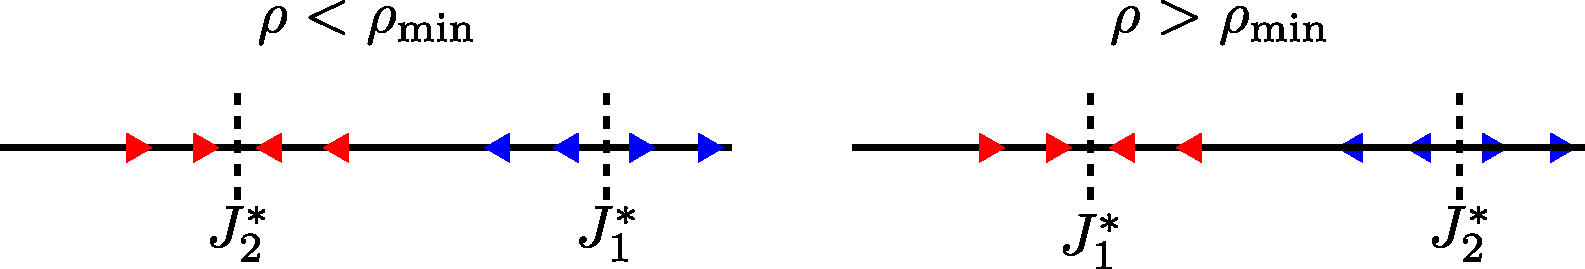
\includegraphics[width=0.45\textwidth]{./rg_flow.pdf}
	\caption{The three fixed points of the overscreened RG equation. Only the intermediate one is stable.}
	\label{rg_flow}
\end{figure}

The RG equation reduces to the perturbative form \(\Delta J_{(j)} \simeq \frac{J_{(j)}^2 \mathcal{N}_{(j)}}{D_{(j)}}\left( 1 - \frac{1}{2}\rho J_{(j)} K \right)\)~\cite{Kogan_2018,Kuramoto1998,Noz_blandin_1980,tripathi2018landau} when one replaces \(\omega_j\) with the ground state energy \(-\frac{D_{(j)}}{2}\) and assumes \(J \ll D_{(j)}\).

\subsection{Star graph as the effective fixed point Hamiltonian}
The fixed point Hamiltonian takes the form
\begin{equation}\begin{aligned}
	H^* = \sum_l\left[ \sum^*_{k}\epsilon_{k,l} \hat n_{k\alpha,l} + J\sum_{kk^\prime}^* \vec{S_d}\cdot\frac{1}{2}\vec{\sigma}_{\alpha\alpha^\prime}c_{k\alpha,l}^\dagger c_{k^\prime\alpha^\prime, l}~.\right]
\end{aligned}\end{equation}
We have not explicitly written the decoupled degrees of freedom \(D_{(j)} > D^*\) in the Hamiltonian. The \(*\) over the summations indicate that only the momenta inside the window \(D^*\) enter the summation. There is an implied summation over the spin indices \(\alpha,\beta\).

To study the low energy physics and universality of the problem, we will mostly focus on the zero bandwidth limit of the fixed point Hamiltonian. Upon setting the chemical potential equal to the Fermi energy, this zero bandwidth model becomes a Heisenberg spin-exchange Hamiltonian.
\begin{equation}\begin{aligned}
	\label{stargraph}
	H^* = J\sum_l\sum_{kk^\prime}^* \vec{S_d}\cdot\frac{1}{2}\vec{\sigma}_{\alpha\alpha^\prime}c_{k\alpha,l}^\dagger c_{k^\prime\alpha^\prime, l} = J\vec{S_d}\cdot\sum_l \vec{s}_l~.
\end{aligned}\end{equation}
At the last step, we defined the local spin operator of each conduction channel \(\vec{s}_l = \frac{1}{2}\sum_{kk^\prime}^*\sum_{\alpha\beta}\vec{\sigma}_{\alpha\alpha^\prime}c_{k\alpha,l}^\dagger c_{k^\prime\alpha^\prime, l}\).
\begin{figure}[htpb]
	\centering
	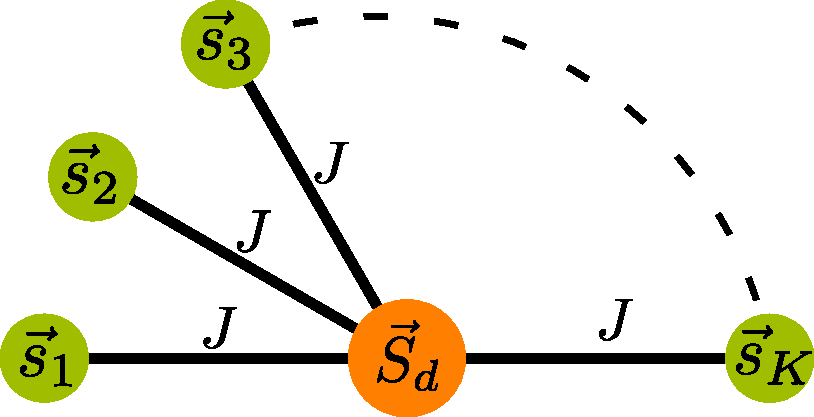
\includegraphics[width=0.45\textwidth]{./stargraph.pdf}
	\caption{Zero bandwidth limit of the fixed point Hamiltonian. The central yellow node is the impurity spin, which is talking withe the local spins of the channels represented as green nodes.}
	\label{fig:-stargraph-pdf}
\end{figure}

There are multiple reasons for working with specifically the star graph and zero mode Hamiltonians in general. In the URG analysis of the one dimensional Hubbard model \cite{1dhubjhep}, a study of the zero mode Hamiltonian (in that case, the Fermi surface itself) was sufficient to topologically characterize various phases of the Berezinskii-Kosterlitz-Thouless (BKT) RG phase diagram. In the single-channel Kondo model, the star graph is just the two spin Heisenberg, and they share the same ground state \cite{varma_yafet_1976,yosida_1966,wilson1975renormalization} along with thermodynamic properties \cite{varma_yafet_1976,kondo_urg}. Within the MCK model itself, the star graph is able to mimic the nature of the RG flows: At weak coupling \(J \to 0^+\), the central spin is weakly coupled to the outer spins and  prone to screening because of the \(s^\pm\) terms in the star graph, and at strong coupling \(J \to \infty^-\), the outer spin-half objects tightly bind with the central spin-half object to form a single spin object that interacts with the remaining states through an exchange coupling which is RG relevant, rendering both the terminal fixed points unstable. The true stable fixed point must then lie somewhere in between, and we recover the schematic phase diagram of fig.~\ref{rg_flow}. Our claim is that the non-Fermi liquid arises solely from the degeneracy of the ground state manifold of the underlying zero mode Hamiltonian, and the star graph captures the degeneracy in its entirety. The RG flows of the MCK model have been show to \textit{preserve the degeneracy of the ground state}~\cite{pang_cox_1991,kroha_kolf_2007,zitko_fabrizio_2017}\textcolor{red}. The star graph conserves the total spin \(S^z\), and this leads to a \(K-\)fold degeneracy in the ground state of the \(K-\)channel spin-half star graph which is preserved under the RG flow. This is qualitatively different from the case of the single-channel Kondo model where the \(2-\)fold degeneracy of the local moment fixed point crosses over into a stable and unique singlet ground state. The importance of the degeneracy can be shown in the following manner. The ground state degeneracy of the more general star graph with a spin-\(S\) impurity and \(K\) channels is given by \(|K - 2S|+1\). The cases of \(K=2S\), \(K<2S\) and \(K>2S\) correspond to exactly screened, underscreened and overscreened regimes respectively. The latter two cases correspond to a multiply-degenerate manifold, and simultaneous have non-Fermi liquid phases~\cite{Noz_blandin_1980,Gan_Andrei_Coleman_1993,emery_kivelson,Gan_mchannel_1994,Tsvelick_Weigmann_mchannel_1984,Tsvelick_weigmann_mchannel_1985,parcollet_olivier_large_N,kimura_taro_Su_N_kondo,PhysRevB.73.224445,cox_jarrell_two_channel_rev,affleck_1991_overscreen,Coleman_tsvelik,affleck1993exact,coleman_pepin_2003,roch_nicolas_costi_2009,schiller_avraham_2008,Durganandini_2011}, while the first regime has a unique ground state and is described by a local Fermi liquid phase \cite{wilson1975,nozieres1974fermi,Noz_blandin_1980,andreiKondoreview,tsvelickKondoreview}, thereby substantiating the claim that a degeneracy greater than unity leads to non-Fermi liquid physics.
\section{Important Properties of the Star Graph}
\subsection{Spectral and Quantum-mechanical features}

\subsection{Measures of entanglement}

\subsection{Twist operators and Gauge theories}

\subsection{Impurity magnetization and susceptibility: Signatures of quantum criticality}
The channel isotropic MCK model is critical; any perturbation away from the perfectly symmetric model in terms of anisotropy is relevant [\textcolor{red}{NEEDS CITATION}]. This critical nature leads to several signatures that can be obtained directly from the star graph. These signatures include a discontinuity in the impurity magnetization at zero temperature in the limit of the external field going to zero, and a diverging susceptibility as temperature goes to zero.

We insert a magnetic field that acts only on the impurity and then diagonalize the Hamiltonian.
\begin{align}
	\label{stargraph_field_hamiltonian}
	H(h) = J^* \vec{S_d}\cdot\vec{s}_\text{tot} + h S_d^z
\end{align}
The Hamiltonian commutes with \(s_\text{tot}\), so it is already block-diagonal in terms of the eigenvalues \(M\) of \(s_\text{tot}\). \(M\) takes values in the range \(\left[M_\text{min}, M_\text{max}\right]\), where \(M_\text{max} = K/2\) for a \(K-\)channel Kondo model, and \(M_\text{min} = 0\)  if \(K\) is even, otherwise \(\frac{1}{2}\). Within each block, the Hamiltonian splits into independent \(2\times 2\) blocks characterized by eigenvalues of the total spin operator \(J^z = S_d^z + s^z_\text{tot}\). Defining \(\alpha = \frac{1}{2}\left(Jm + h\right) + \frac{J}{4}\) and \(x^M_m = M(M+1) - m(m+1)\), the partition function can be written as
\begin{align}
	Z(h) =\sum_{M=M_\text{min}}^{M_\text{max}}r^K_M\left[\sum_{m=-M, \atop{m\in \mathbb{Z}}}^{M-1}2e^{\beta \frac{J}{4}}\cosh \beta\sqrt{J^2x^M_m/4 + \alpha^2} \right.\nonumber\\
\left.+ 2e^{-\beta JM/2}\cosh \beta h/2\right]
\end{align}
Here, \(\beta = \frac{1}{k_B T}\), \(M\) sums over the eigenvalues of \(s_\text{tot}\) while \(m\) sums over \(J^z - \frac{1}{2}\) and the additional degeneracy factor \(r^K_M\) arises from the possibility that there are multiple subspaces defined by \(s_\text{tot}=M\). This multiplicity is given by
\begin{align}
	\label{extra_degen}
	r^K_M = {}^{K-1}C_{K/2 - M}
\end{align}

To calculate the impurity magnetic susceptibility, we will use the expression
\begin{align}
	\chi = \frac{1}{\beta}\lim_{h \to 0}\left[\frac{Z(h)^{\prime\prime}}{Z(h)} - \left(\frac{Z(h)^{\prime}}{Z(h)}\right)^2 \right] 
\end{align}
where the \(\prime\) indicates derivative with respect to \(h\). For brevity, we define \(\theta_M = \beta J (M+\frac{1}{2})/2\) and \(\Sigma_M = \sum_{m=-M, \atop{m\in \mathbb{Z}}}^{M-1}(m+\frac{1}{2})^2\). The derivatives are
\begin{align}
	\lim_{h \to 0}Z(h) &= \sum_{M=M_\text{min}}^{M_\text{max}}r^K_M\left[4Me^{\beta \frac{J}{4}}\cosh \theta_M + 2e^{-\beta JM/2}\right]\\
	\lim_{h \to 0}\frac{\:\mathrm{d}Z(h)}{\:\mathrm{d}h} &=  0\\
	\lim_{h \to 0}\frac{\:\mathrm{d}^2Z(h)}{\:\mathrm{d}h^2} &= \frac{\beta^2}{2}\sum_{M=M_\text{min}}^{M_\text{max}}r^K_M\left[\frac{e^{\beta \frac{J}{4}}}{\theta_M}\left(2M\sinh \theta_M + \right.\right.\nonumber\\
								 &\left.\left.\frac{\beta^2 J^2}{4}\left[\frac{\cosh\theta_M}{\theta_M} - \frac{\sinh \theta_M}{\theta_M^2}\right]\Sigma_M\right)+ e^{-\beta JM/2}\right]
\end{align}
At low temperature \(\beta \to \infty\), only the highest value \(M_\text{max}\) will survive:
\begin{align}
	Z &\to 2 r^K_{M_\text{max}} M_\text{max} e^{\beta \frac{J}{2}(M_\text{max} + 1)}\\
	Z^{\prime \prime} &\to r^K_{M_\text{max}}\left(\frac{\beta }{2(M_\text{max} + \frac{1}{2})}\right)^2 e^{\beta \frac{J}{2}(M_\text{max} + 1)}\Sigma_{M_\text{max}}\\
	\chi &\to \frac{\beta\Sigma_\text{max}}{2M_\text{max}\left(2M_\text{max}+1\right)^2} = \frac{\beta(K-1)}{12(K+1)}
\end{align}

This non-analyticity in a response function is a signature of the critical nature of the Hamiltonian. This is in contrast to the behaviour in the non-critical exactly-screened fixed point where the ground state is unique. There, the susceptibility becomes constant at low temperatures: \(\chi(T\to 0) = \frac{W}{4 T_K}\), \(T_K\) being the single-channel Kondo temperature and \(W\) the Wilson number \cite{wilson1975renormalization,nozieres1974fermi,bullaNRGreview,kondo_urg}.

Another non-analyticity arises when we consider the impurity free energy and the magnetization. The thermal free energy is given by
\begin{equation}\begin{aligned}
	F(h) = -\frac{1}{\beta}\ln Z(h) = -\frac{1}{\beta}\ln\sum_{E_n}e^{-\beta E_n}
\end{aligned}\end{equation}
At \(T \to 0\), only the most negative energy \(E_\text{min}\) survives. Assuming a non-degenerate ground state for \(h \neq 0\), the zero temperature free energy becomes
\begin{equation}\begin{aligned}
	F(h\neq 0, T\to 0) = -\frac{1}{\beta}\ln e^{-\beta E_\text{min}} = E_\text{min}
\end{aligned}\end{equation}
In the star graph Hamiltonian with \(K-\)channels and in the presence of a field on the impurity (eq.~\ref{stargraph_field_hamiltonian}), the ground state energy will be one of the negative eigenvalues:
\begin{equation}\begin{aligned}
	\lambda^{M,h}_{m, -} = -J/4 - \frac{1}{2}\sqrt{J^2(M+1/2)^2 + h^2 + 2hJ(m+1/2)}
\end{aligned}\end{equation}
The minimum eigenvalue is obtained by maximizing \(h(m+1/2)\). For \(h>0\), the ground state is renormalized for the most positive value of \(m\), which is \(M-1\). On the other hand, for \(h<0\), it occurs for \(m=-M\), because that is the most negative value it can take. Among all the values of \(M\), the global ground state is at the largest value of \(M\), \(K/2\). Therefore, the minimal energy eigenvalue is
\begin{equation}\begin{aligned}
	E_\text{min} = -J/4 - \frac{1}{2}\sqrt{J^2(K+1)^2/4 + h^2 + |h|J(K-1)}
\end{aligned}\end{equation}
The first derivative of the free energy with respect to the field gives
\begin{equation}\begin{aligned}
	F^\prime(h\neq 0, T\to 0) =- \frac{2h + J(K-1)\text{sign}(h)}{4\sqrt{\frac{J^2}{4}(K+1)^2 + h^2 + |h|J(K-1)}}
\end{aligned}\end{equation}
There we used the result that the derivative of \(|x|\) is \(\text{sign}(x)\). If we now take \(h\) to zero from both directions, we get the magnetization of the impurity
\begin{equation}\begin{aligned}
	m = F^\prime(h \to 0^\pm, T\to 0) = \mp \frac{1}{2}\frac{(K-1)}{(K+1)}
\end{aligned}\end{equation}

The magnetization is therefore discontinuous as \(h\to 0\); it goes to different values depending on the direction in which we take the limit. The only case where it is not analytic is when \(K=1\); then the derivative goes to zero from both directions. This non-analyticity has also been verified numerically.
\begin{figure}[!htpb]
	\centering
	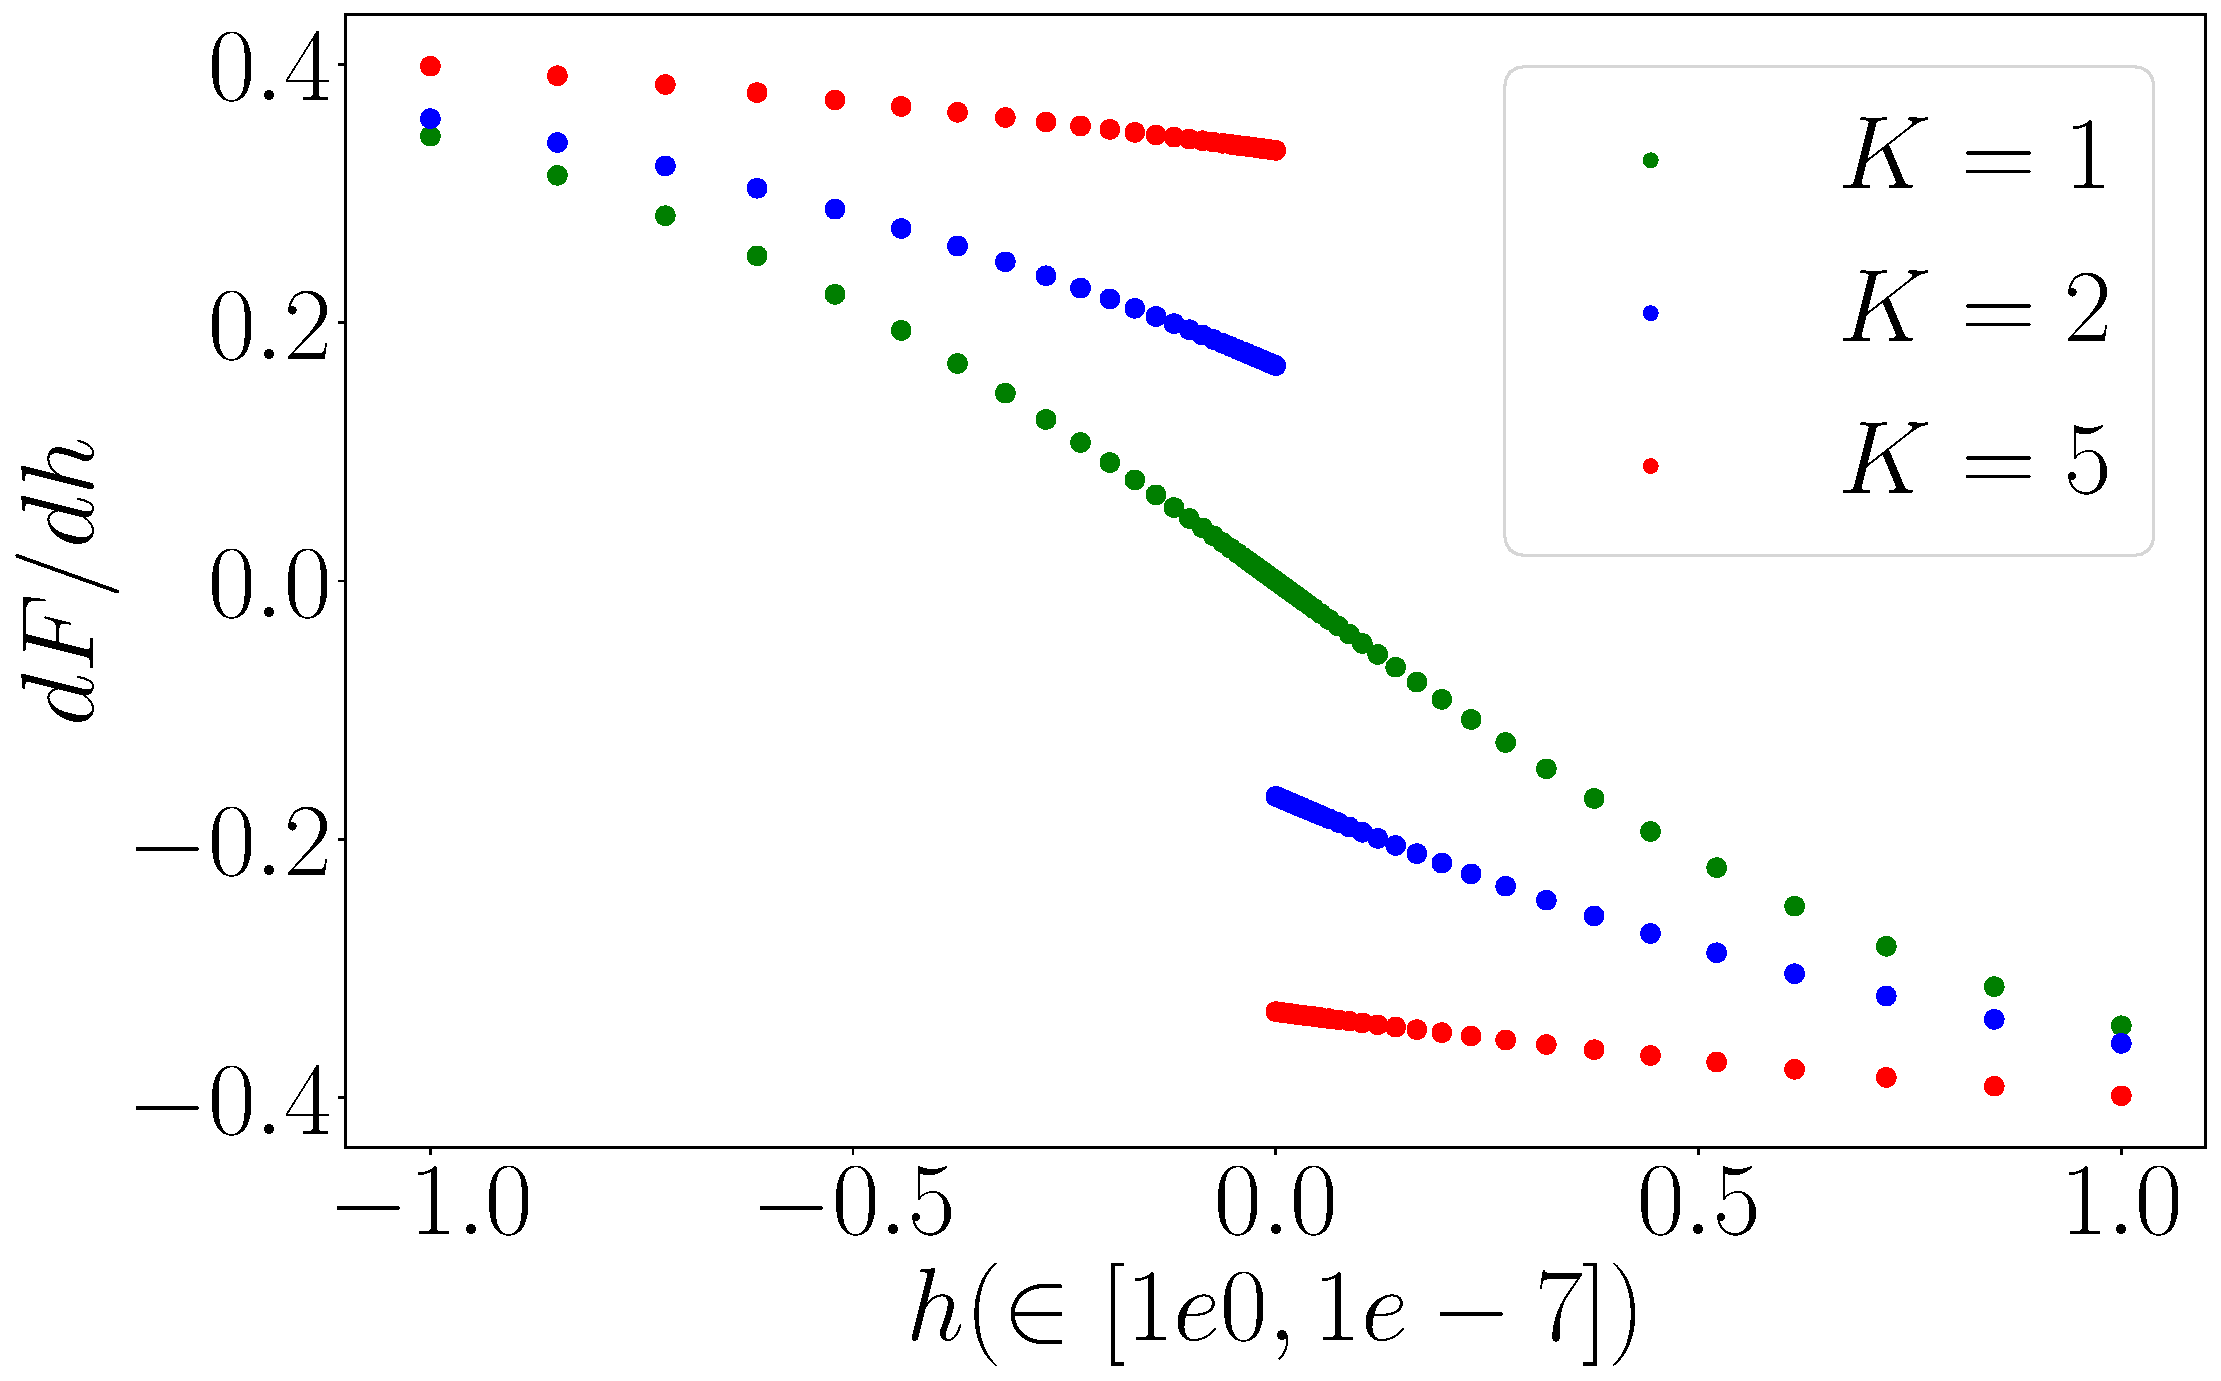
\includegraphics[width=0.45\textwidth]{../numerics/disc_mag_imp.pdf}
	\caption{Non-analytic free energy for \(K>1\) and analytic free energy for \(K=1\).}
\end{figure}

The non-analyticity for \(K>1\) occurs because the magnetic field is able to flip the ground state. For example, for \(K=2\), the states in question are \(\ket{M=1, m=-1,0}\). For \(h>0\), the ground state occurs in the subspace \(\ket{S_d^z=1/2, m=-1},\ket{S_d^z=-1/2,m=0}\). If we now flip the magnetic field, the ground state subspace flips to \(\ket{S_d^z=1/2, m=0},\ket{S_d^z=-1/2,m=1}\). Instead, if we look at the case of \(K=1\), the ground state is in the subspace of \(\ket{S_d^z=1/2,m=-1/2},\ket{S_d^z=-1/2, m=1/2}\), and since there is only this one subspace, the ground state is independent of the field. From this discussion, it is clear that the non-analyticity appears because there are multiple values of \(m \in [-M, M-1]\) in the ground state manifold, which means that it is the ground state degeneracy that causes the non-analyticity.

\subsection{Impurity magnetization in terms of parity operators}

\section{Effect of conduction bath excitations on the fixed point theory}
\subsection{Non-Fermi liquid effective Hamiltonian}

\subsection{Low temperature thermodynamic behaviour}

\subsection{Non-Fermi liquid signatures in momentum space}
Obtaining the effective Hamiltonian involves obtaining the low energy excitations on top of the ground state of the star graph. The large-energy excitations are ones that involve spin flips. This guides the separation of the Hamiltonian into a diagonal and an off-diagonal piece:
\begin{align}
	H = H_d + V = \underbrace{H_0 + J S_d^z s_\text{tot}^z}_{H_d} + \underbrace{\frac{J}{2}S_d^+ s_\text{tot}^- + \text{h.c.}}_{V + V^\dagger}
\end{align}
We define \(V\) as the interaction term that decreases \(s_\text{tot}^z\) by 1: \(V \ket{s_\text{tot}^z} \to \ket{s_\text{tot}^z - 1}\). Similarly, we define \(V^\dagger \ket{s_\text{tot}^z} \to \ket{s_\text{tot}^z + 1}\). The effective Hamiltonian that has the states \(\ket{S_d^z, s_\text{tot}, s_\text{tot}^z}\) as eigenstates are
\begin{widetext}
\begin{align}
	H_\text{eff} = H_d + V \frac{1}{E_\text{gs} - H_d}V = H_d + \frac{J}{2}S_d^+ s_\text{tot}^- \frac{1}{E_\text{gs} - J S_d^z s_\text{tot}^z - H_0}\frac{J}{2}S_d^- s_\text{tot}^+ +\frac{J}{2}S_d^- s_\text{tot}^+ \frac{1}{E_\text{gs} - J S_d^z s_\text{tot}^z - H_0}\frac{J}{2}S_d^+ s_\text{tot}^-
\end{align}
This is obtained from the Schrodinger equation for the ground state. If we expand the ground state in terms of \(\ket{S_d^z, s_\text{tot}, s_\text{tot}^z}\), we have  \(\ket{\Psi_\text{gs}} = \sum_{S_d^z, s_\text{tot},s_\text{tot}^z}C_{S_d^z, s_\text{tot},s_\text{tot}^z}\ket{S_d^z, s_\text{tot}, s_\text{tot}^z}\). The Schrodinger equation for the ground state can be written as
\begin{align}
	E_\text{gs}\ket{\Psi_\text{gs}} = H \ket{\Psi_\text{gs}} = \left(H_d + V\right)\ket{\Psi_\text{gs}} \implies \left(E_\text{gs} - H_d\right)\sum C_{S_d^z, s_\text{tot},s_\text{tot}^z}\ket{S_d^z, s_\text{tot}, s_\text{tot}^z} = V\sum C_{S_d^z, s_\text{tot},s_\text{tot}^z}\ket{S_d^z, s_\text{tot}, s_\text{tot}^z}
\end{align}
\end{widetext}
\textcolor{red}{\(E_\text{gs}\) is the ground state energy, and can be replaced by the star graph ground state energy if we remove the kinetic energy cost via normal ordering: \(E_\text{gs} = \)}. Since \(V\) only changes \(S_d^z \to -S_d^z\) and \(s^z_\text{tot} \to s^z_\text{tot} \pm 1\), we can simplify the equation into individual smaller equations. For the two-channel model, the possible states are \(s_\text{tot},s^z_\text{tot} = (0,0), (1,-1), (1,0), (1,1)\). The individual equations for these states are
\begin{align}
	\label{eff_ham_Sdz_10}
	E_\text{gs} \ket{\frac{1}{2}, 1, 0} &= \left(H_d + V \frac{1}{E_\text{gs} - H_d}V^\dagger\right) \ket{\frac{1}{2}, 1, 0}\\
	E_\text{gs} \ket{-\frac{1}{2}, 1, 0} &= \left(H_d + V^\dagger \frac{1}{E_\text{gs} - H_d} V\right) \ket{-\frac{1}{2}, 1, 0}\\
\end{align}
These equations represent the Schrodinger equation for the states \(\ket{S_d^z, 1, 0}\), and the right hand sides therefore give the effective Hamiltonians for those states. If we combine the states into a single subspace \(\ket{1,0}= \left\{\ket{\frac{1}{2}, 1, 0}, \ket{-\frac{1}{2}, 1, 0}\right\}\), the effective Hamiltonian for this composite subspace becomes the sum of the two parts:
\begin{align}
	\label{eff_ham_10}
	H^{1,0}_\text{eff}\ket{1, 0}\bra{1, 0} = \left(H_d + V G_0 V^\dagger + V^\dagger G_0  V\right) \ket{1, 0}
\end{align}
where \(G_0 = \left(E_\text{gs} - H_d\right)^{-1}\). If we expand the subspace as \(\ket{1,0} = \ket{\frac{1}{2}, 1, 0} + \ket{-\frac{1}{2}, 1, 0}\), we recover eqs.~\ref{eff_ham_Sdz_10}. Solving similarly for the other states gives
\begin{align}
	H^{1,1}_\text{eff}\ket{1,  1}\bra{1,  1} &= \left(H_d + V^\dagger G_0  V\right) \ket{1,  1}\\
	H^{1,-1}_\text{eff}\ket{1, - 1}\bra{1, - 1} &= \left(H_d + V G_0 V^\dagger\right) \ket{1, - 1}
\end{align}

To calculate these effective Hamiltonians, we will calculate the individual terms. We can easily simplify the \(S_d^z\) in the denominator of \(G_0\), because \(S_d^\pm \frac{1}{A + B S_d^z} = S_d^\pm \frac{1}{A \mp \frac{1}{2}B}\):
\begin{align}
	V G_0 V^\dagger = \frac{J^2}{4} s_\text{tot}^- \frac{\frac{1}{2} + S_d^z}{E_\text{gs} + \frac{J}{2} s_\text{tot}^z - H_0} s_\text{tot}^+ \\
	V^\dagger G_0 V = \frac{J^2}{4} s_\text{tot}^+ \frac{\frac{1}{2} - S_d^z}{E_\text{gs} - \frac{J}{2} s_\text{tot}^z - H_0} s_\text{tot}^-
\end{align}
Since \(H_0\) does not commute with the spin operators, we will need to expand the denominator to make sense of this Hamiltonian.
\begin{widetext}
\begin{align}
	 V G_0 V^\dagger =  s_\text{tot}^- \frac{1}{E_\text{gs} + \frac{J}{2} s_\text{tot}^z}\left[1 + \frac{1}{E_\text{gs} + \frac{J}{2} s_\text{tot}^z}H_0 + \frac{1}{E_\text{gs} + \frac{J}{2} s_\text{tot}^z}H_0\frac{1}{E_\text{gs} + \frac{J}{2} s_\text{tot}^z}H_0 + \ldots\right] s_\text{tot}^+\\
	 V^\dagger G_0 V =  s_\text{tot}^+ \frac{1}{E_\text{gs} - \frac{J}{2} s_\text{tot}^z}\left[1 + \frac{1}{E_\text{gs} - \frac{J}{2} s_\text{tot}^z}H_0 + \frac{1}{E_\text{gs} - \frac{J}{2} s_\text{tot}^z}H_0\frac{1}{E_\text{gs} - \frac{J}{2} s_\text{tot}^z}H_0 + \ldots\right] s_\text{tot}^-
\end{align}
\end{widetext}
This is an expansion in \(H_0^n/J^{n+1}, n=0,1,2,\ldots\). Expanding up to \(n=2\) and keeping at most two particle interaction terms, 
the effective Hamiltonians for these states are:
\begin{widetext}
\begin{align}
	H_\text{eff}^{1, 1} &= H_0 + J S_d^z + \frac{J^2}{4}\frac{2}{E_\text{gs}}\left[1 + \frac{H_0}{E_\text{gs}} + \frac{s^+_\text{tot}X_{1,\text{tot}}}{2 E_\text{gs}} + \frac{H_0^2 }{E_\text{gs}^2} - \frac{Z_{1,\text{tot}} H_0}{E_\text{gs}^3}\right] \left(\frac{1}{2} - S_d^z\right) \\
	H_\text{eff}^{1, -1} &= H_0 - J S_d^z + \frac{J^2}{4}\frac{2}{E_\text{gs}}\left[1 + \frac{H_0}{E_\text{gs}}  - \frac{s^-_\text{tot}X^\dagger_{1,\text{tot}}}{2 E_\text{gs}}  + \frac{H_0^2}{E_\text{gs}^2}  - \frac{ Z_{1,\text{tot}} H_0}{E_\text{gs}^3}\right] \left(\frac{1}{2} + S_d^z\right) \\
	H_\text{eff}^{1, 0} &= H_0 + \frac{J^2}{2\left(E_\text{gs} + \frac{J}{2}\right)}\left[1 + \frac{ H_0 + \left(\frac{1}{2} + S_d^z\right) s^+_\text{tot}X_{1,\text{tot}} - \left(\frac{1}{2} - S_d^z\right) s^-_\text{tot}X^\dagger_{1,\text{tot}}}{2 \left(E_\text{gs} + \frac{J}{2}\right)} + \frac{H_0^2}{\left(E_\text{gs} + \frac{J}{2}\right)^2} - \frac{Z_{1,\text{tot}} H_0}{\left(E_\text{gs} + \frac{J}{2}\right)^3} \right]
\end{align}
\end{widetext}
We employed the definitions \(X_{n,\text{tot}} \equiv  \sum_l \sum_{k,k^\prime}\left(\epsilon_k - \epsilon_{k^\prime}\right)^n c^\dagger_{k \downarrow}c_{k^\prime \uparrow},  X_{n,l}\) and \( Z_{1,\text{tot}} \equiv \sum_{k,k^\prime,l}\left( \epsilon_k - \epsilon_{k^\prime} \right) \frac{1}{2}\left(c^\dagger_{k \uparrow,l}c_{k^\prime \uparrow,l} - c^\dagger_{k \downarrow,l}c_{k^\prime \downarrow,l}\right)\). Focusing on the effective Hamiltonian for \(\left( 1,0 \right) \), we see lots of non-Fermi liquid terms of the form \(s^+_\text{tot}X_{1,\text{tot}}, s^-_\text{tot}X^\dagger_{1,\text{tot}},Z_{1,\text{tot}} H_0\). These arise because of the degenerate manifold and the increased availability of states in the Hilbert space for scattering, as compared to the unique singlet ground state of the single-channel Kondo model.


\section{Strong-weak duality of the general spin-\(S\) impurity multi-channel Kondo model}
We start from a strong coupling \((J \to \infty)\) spin-\(S\) impurity MCK Hamiltonian in the over-screened regime \(\left( K > 2S \right) \),
\begin{equation}\begin{aligned}
	\label{strong_ham}
	H(J) = \sum_{k,\sigma,l}\epsilon_{k,l} \hat n_{k\sigma,l} + J \vec{S_d}\cdot\vec{s}_\text{tot}~.
\end{aligned}\end{equation}
Here, \(\vec s_\text{tot}\) is the total spin \(\sum_l \sum_{kk^\prime \alpha\beta} \vec \sigma_{\alpha\beta}c^\dagger_{k\alpha,l}c_{k^\prime\beta,l}\) of all the zero modes. At strong-coupling, the ground states of the star graph eq.~\ref{stargraph} act as a good starting point for a perturbative expansion. As argued previously, there are \(K-2S+1\) ground states, labeled by the \(K\) values of the total spin angular momentum \(S^z = S_d^z + s_\text{tot}^z = -\frac{K}{2} + S, -\frac{K}{2} + S + 1, \ldots, \frac{K}{2} - S\). To leverage the large coupling, one can define a new spin impurity \(\mathbb{S}\) out of this ground state manifold. Since the degeneracy of a spin is given by its multiplicity \(2S^\prime + 1\), we have \(2S^\prime + 1 = K-2S+1 \implies S^\prime = \frac{K}{2} - S\). That is, the spin-\(S\) impurity has a dual described by a spin-\((K-2S+1)\) impurity. The states of this new spin are defined by
\begin{gather}
	\mathbb{S}_d^z \ket{S^z} = S^z \ket{S^z},\nonumber\\
	\mathbb{S}_d^\pm \ket{S^z} = \sqrt{S^\prime\left( S^\prime + 1 \right) - S^z\left( S^z \pm 1\right)} \ket{S^z \pm 1}
\end{gather}
The excited states of the star graph can be used to define bosons \cite{kroha_kolf_2007}, and the hopping into the lattice can then be re-written using these Bosons. One can then remove the single-particle hoping between the zero modes and the first sites using a Schrieffer-Wolff transformation in the small coupling \(J^\prime = \gamma \frac{4t^2}{J}\), and generate an exchange-coupling between the new impurity \(\vec {\mathbb{S}}_d\) and the new zero modes formed out of the remaining sites in the lattice \cite{kroha_kolf_2007} (by remaining, we mean those real space sites that have not been consumed into forming the new spin). The new Hamiltonian, characterized by the small super-exchange  coupling \(J^\prime\), has the form
\begin{equation}\begin{aligned}
	H^\prime(J^\prime) = \sum_{k,\sigma,l}\epsilon_{k,l} \hat n_{k\sigma,l} + J^\prime \vec{\mathbb{S}_d}\cdot\vec{s^\prime}_\text{tot}
\end{aligned}\end{equation}
The prime on \(s_\text{tot}\) indicates that it is formed by the new zero modes. This Hamiltonian is very similar to the one in eq.~\ref{strong_ham}, and that is the essence of the strong-weak duality: One can go from the over-screened strong coupling spin-\(S\) MCK model to another over-screened weak coupling spin-\((K-2S+1)\) MCK model. For the case of \(K=4S\), we have \(S^\prime = S\), and both \(S_d\) and \(\mathbb{S}_d\) describe the same spin objects (at least formally). The two models are then said to be self-dual. For example, for the case of spin-half MCK model, two-channel model is self-dual.

One important consequence of the duality relationship between the two overscreened models is that the RG equations are also dual; while the strong coupling model has an irrelevant coupling \(J\) that flows down to the intermediate fixed point \(J^*\), the weak coupling model has a relevant coupling \(J^\prime\) that flows up to the same fixed point \({J^\prime}^* = J^*\). From the RG equation for the general spin-\(S\) MCK model, we know that \({J^\prime}^* = \frac{2}{K \rho^\prime}\), where \(\rho^\prime\) is the DOS for the bath of the weak coupling Hamiltonian. This constrains the form of the scaling factor \(\gamma\):
\begin{equation}\begin{aligned}
	{J^\prime}^* = \frac{\gamma 4t^2}{J^*} = \frac{2}{K \rho^\prime} \implies \gamma = \frac{1}{4t^2} {J^*}^2 = \frac{1}{K^2 t^2 \rho \rho^\prime}
\end{aligned}\end{equation}
\begin{figure}[htpb]
	\centering
	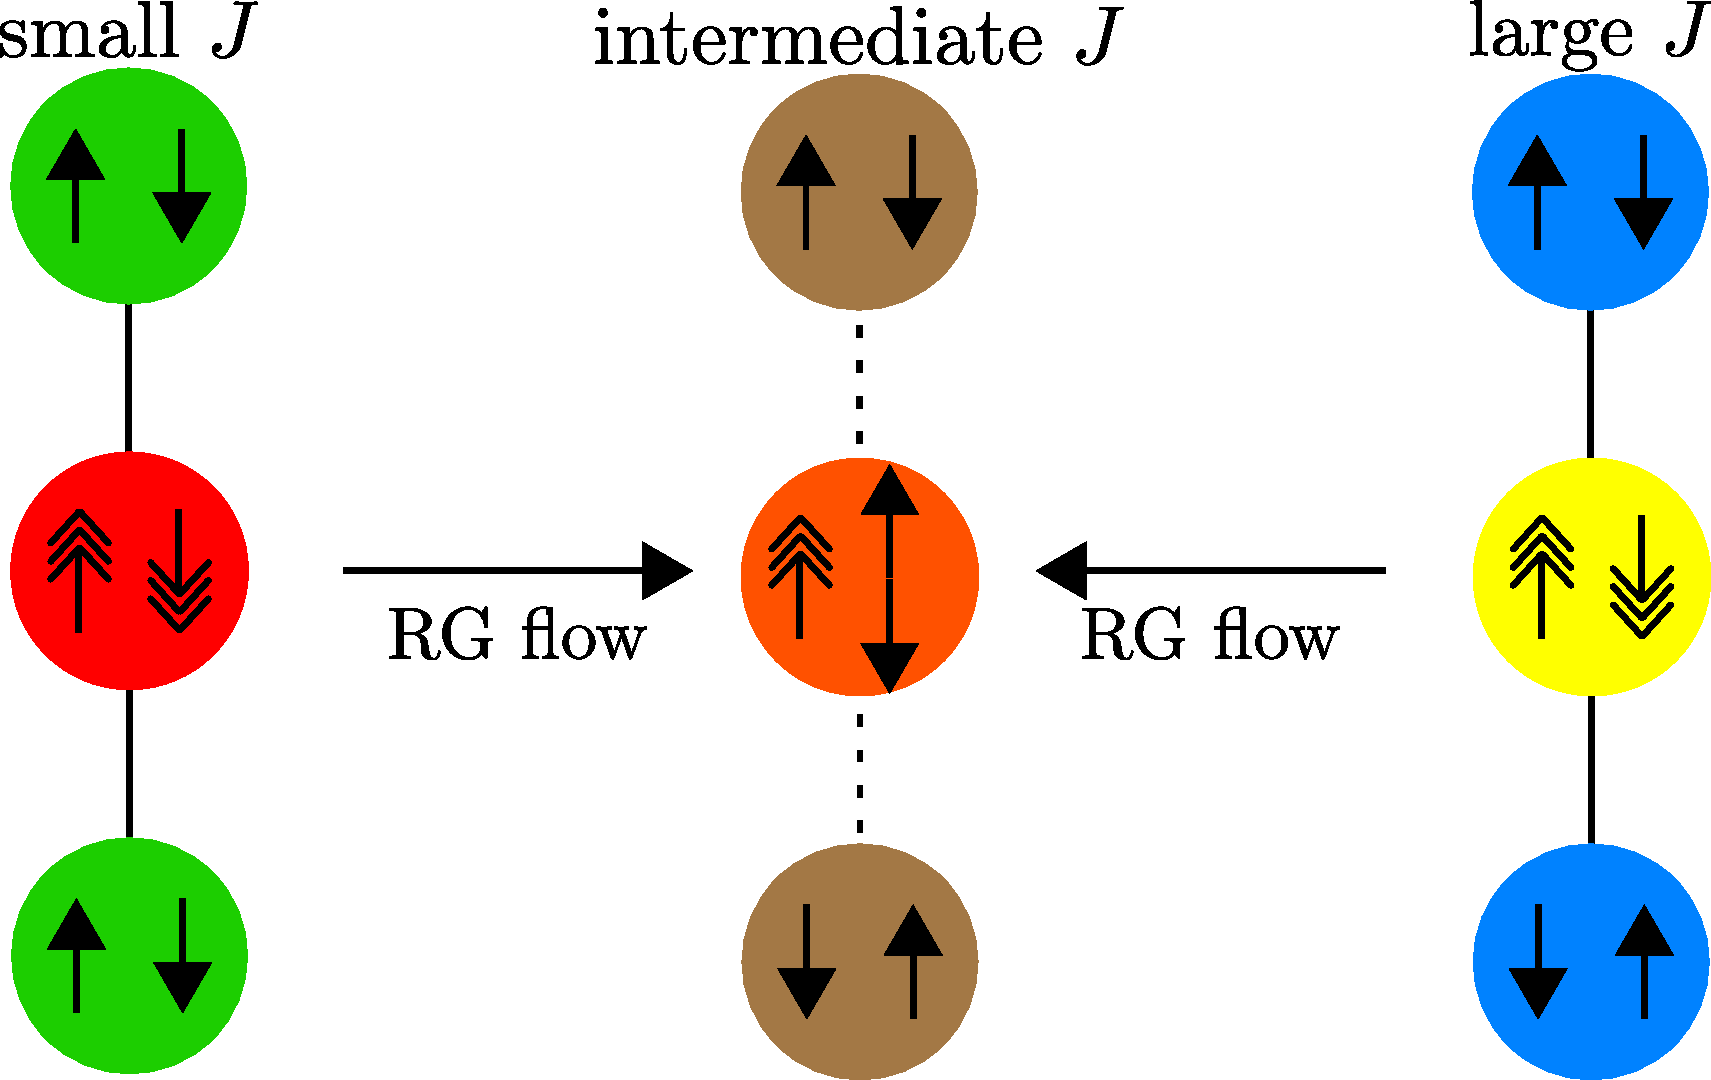
\includegraphics[width=0.45\textwidth]{./duality.pdf}
	\caption{Duality of the RG flows as seen in the star graph Hamiltonian. The red and green circles represent the impurity and zeroth site spins respectively. At large \(J\), the red circle binds with the green circles to form an effective spin \(\frac{K-1}{2}\) object (yellow) that interacts with the remaining spin of the conduction bath (blue circles). The fixed point consists of the red (purple) and green (yellow) circles binding to form a doubly degenerate ground state (orange) that interacts with the star graph of the remaining sites (brown) through the hopping.}
	\label{duality_fig}
\end{figure}


\section{Impurity Quantum Phase transition in the multi-channel Kondo model under channel anisotropy}

\section{Conclusions}


\acknowledgments
The authors thank P. Majumdar, A. Mitchell, S. Sen, S. Patra, M. Mahankali and R. K. Singh for several discussions and feedback. Anirban Mukherjee thanks the CSIR, Govt. of India and IISER Kolkata for funding through a research fellowship. Abhirup Mukherjee thanks IISER Kolkata for funding through a research fellowship. AM and SL thank JNCASR, Bangalore for hospitality at the inception of this work. NSV acknowledges funding from JNCASR and a SERB grant (EMR/2017/005398).

\appendix
\section{URG}
\label{appendix_urg}

\bibliography{mscript_mck}
\end{document}
